\section{Management Summary}
\subsection*{Ausgangslage}
Open Street Map, eine online Kartenanwendung wie Google Maps, bietet seinen Benutzern eine Fussgängernavigation an. Der Nutzer wird entlang von Strassen und Wegen zu seinem Ziel geleitet. Dabei müssen die bestehenden Fussgängerstreifen in die Planung einbezogen werden, damit auch eine Überquerung der Strassen möglich ist. Unglücklicherweise sind Zebrastreifen nur lückenhaft in Open Street Map erfasst, was die Fussgängernavigation ungenau, wenn nicht sogar fehlerhaft macht.

Dieses Projekt ist der Versuch einer automatischen Erkennung von Fussgängerstreifen auf Orthofotos (umgangssprachlich Satellitenbildern). Da das maschinelle Erfassen von Daten in Open Street Map nicht erlaubt ist, müssen die gefundenen Koordinaten in ein Crowdsourcing-System wie Maproulette eingespeist werden. In einem Crowdsourcing-System bewerten Nutzer, ob die eingefügten Daten stimmen oder nicht.
\begin{figure}[H]
	\centering
	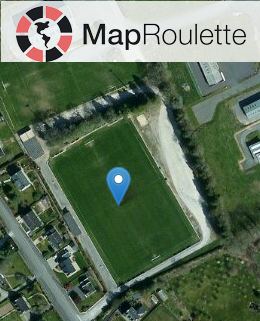
\includegraphics[]{images/Maproulette_management_summary.png}
	\caption[Management Summery Maproulette]{Maproulette Challenge - Befindet sich hier ein Fussballfeld?}
\end{figure}


\subsection*{Ergebnisse}
Aus diesem Projekt entstand einen Applikation für die automatische Erkennung von Fussgängerstreifen. Die Applikation bezieht in einem angegebenen Bereich automatisch die entsprechend Orthofotos und Strasseninformationen und extrahiert die Koordinaten der Fussgängerstreifen. Die Koordinaten werden in einer Json-Datei abgelegt und können in eine Maproulette Challenge umgewandelt werden.
\\
\begin{figure}[H]
	\centering
	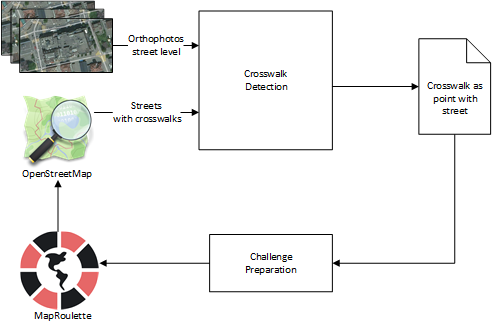
\includegraphics[]{images/management_summary_1.png}
	\caption[Management Summery Überblick]{Überblick}
\end{figure}

\subsubsection{Kennzahlen}
Die Applikation erkannte mehr als 80\% aller gelben Fussgängerstreifen mit einer Fehlerrate von weniger als 10\%. Die Koordinaten der Fussgängerstreifen im Raum des Kanton Zürich, Kanton Zugs und Teile des Kanton St. Gallen konnten an Maproulette zur Einpflegung in Open Street Map übergeben werden
\\
\begin{figure}[H]
	\centering
	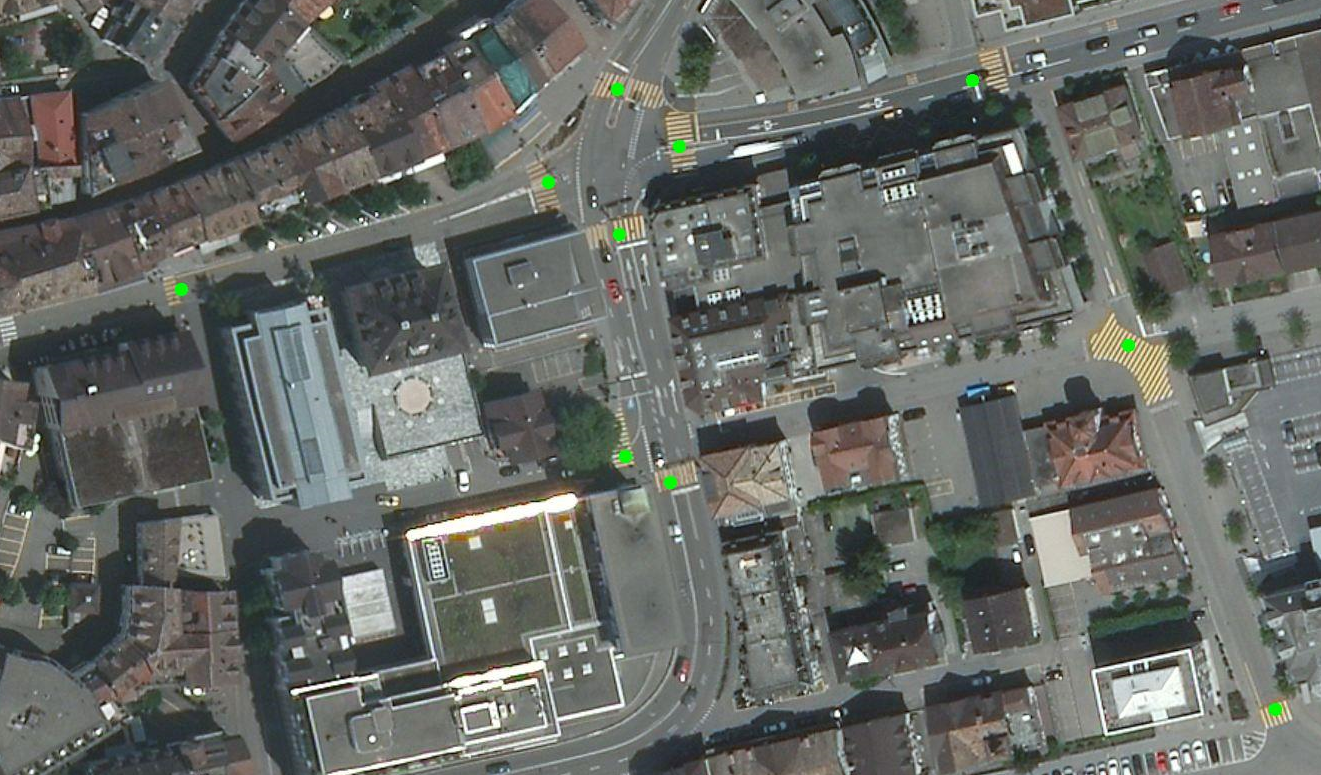
\includegraphics[width=\textwidth -10mm]{images/boxsave_rappi.png}
	\caption[Überblick]{Rapperswil Innenstadt - Gefundene Fussgängerstreifen sind mit einem grünen Punkt markiert.}
\end{figure}

\subsection*{Ausblick}
Der Erkennungsalgorithmus ist zu Ende dieses Projektes auf die Region Zürich und Ostschweiz spezialisiert. Mit weiteren Optimierungen ist es möglich, alle Zebrastreifen in der Schweiz zu erfassen und sogar weisse Zebrastreifen für andere europäische Länder zu erkennen. Auch weitere Strassenmarkierungen sind denkbar.
\newpage